\problemname{Astronom}
\illustration{.3}{img/TychoBrahe.JPG}{}

\noindent
Astronomen elsker stjernekiggeri.
Han får særlig glæde af at betragte $k$~stjerner samtidigt gennem sit teleskop.
At bygge et teleskop med radius~$r$ koster $t \cdot r$~kroner.
Et nybygget teleskop vil pege præcis på origo~$(0,0)$.
At få det at pege et andet sted hen kræver også en indsats;
at flytte teleskopet en afstand på $d$~enheder koster $s \cdot d$ kroner.
Astronomen kan observere alle stjerner med afstand højst~$r$ fra, hvor teleskopet peger.

Hvor meget koster det at bygge og flytte et teleskop, der tillader observation af $k$~stjerner på én gang?

\medskip

Alle koordinater og afstande er angivet i det euklidiske plan.

\section*{Eksempel}

Her er et eksempel med $n=3$ stjerner på positionerne $(0,0)$, $(2,0)$ og $(3,1)$.
Det farvelagte område viser et teleskop med radius $1$, der peger på $(1,0)$ og dækker to stjerner; dette koster $s + t$ kroner og er en optimal løsning på eksempel~$3$ forneden.
Billedet viser desuden optimale løsninger på eksempler~$1$, $2$ og~$4$.

\medskip
\noindent
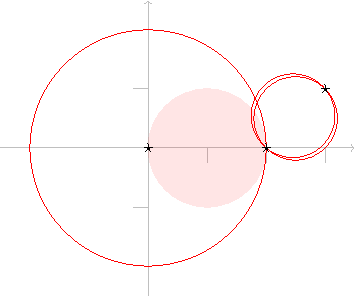
\includegraphics[width=.3\textwidth]{img/samples.pdf}

\section*{Indlæsning}

Første linje består af fire heltal:
antallet $k$ af stjerner, som astronomen ønsker at observere,
antallet $n$ af stjerner på aftenens stjernehimmel,
omkostningen $s$ for at flytte teleskopet og
omkostningen $t$ for at bygge et teleskop.
Derefter følger $n$ linjer, hvor den $i$'te linje indeholder de heltallige koordinater $x_i$ og $y_i$ for den $i$'te stjerne.

\section*{Udskrift}

Et enkelt reelt tal: det mindste beløb i kroner, som astronomen skal bruge.

\section*{Begrænsninger og pointgivning}

Du kan antage at følgende gælder:
\begin{enumerate}
\item $1\leq k\leq n\leq 700$. % constraint:kn
\item $x_i, y_i\in \{-10^9,\ldots, 10^9\}$ for alle $i\in\{1,\ldots,n\}$. % constraint:xy
\item $s,t\in \{0,\ldots, 10^9\}$. % constraint:st
\item Dit svar accepteres hvis det er inden for en relativ eller absolut tolerance på $\epsilon = 10^{-6}$ af det korrekte svar.
\end{enumerate}

Din løsning vil blive testet på en række testgrupper, hver med en vist antal point.
Hver testgruppe indeholder en række testfald.
For at opnå point for en testgruppe skal du løse alle testfald i testgruppen.
Din endelige score vil være den højeste score for en enkelt indsendelse.

\medskip
\noindent
\begin{tabular}{lll}
Gruppe & Point & Begrænsninger\\\hline
$1$ & $8$ & $t\leq s$\\
$2$ & $9$ & $n\leq 50$ og $s=0$\\
$3$ & $18$ & $s=0$\\
$4$ & $13$ & $n\leq 50$\\
$5$ & $14$ & $n\leq 350$\\
$6$ & $15$ & $\epsilon = 1/10$\\
$7$ & $23$ & \emph{Ingen yderligere begrænsninger}
\end{tabular}
